


This week I tried to make some progress with regarding the pressure mapping, rotational stiffness determination and some thesis writing. However, I did not manage to completely work out all the results in a nice and structured manner. Partly because some parts such as, the pressure mapping and rotational stiffness determination are still a little "uncertain" or not complete. 

I have tried to find some force to pressure mapping. I have done this now for only the elongation part. I put a force at the top of the actuator, and let abaqus solve it. My reasoning was that a pressure on top of the actuator will result in the same deformation as putting the bellows under pressure. I ran some simulations and used optimization to find the mapping parameter $\alpha$ as in : $F = \alpha p$ as seen in Figure \ref{fig:pressure}. Here $\alpha$ was found to be equal to $0.3118$. We should discuss whether this approach is valid, and if so, think of doing the same for the rotation.


\begin{figure}[H]
    \centering
    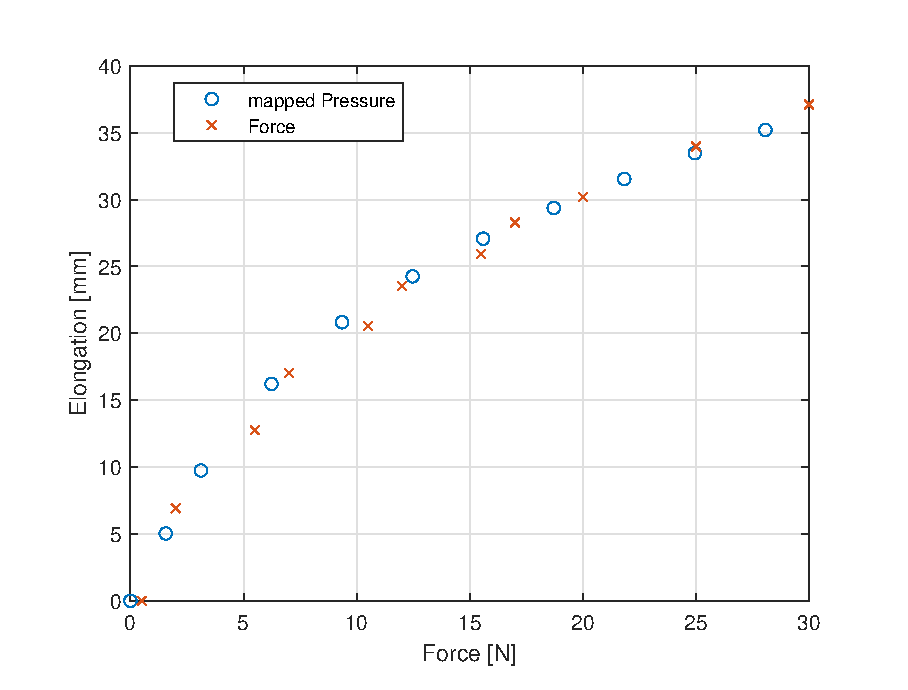
\includegraphics[width = 0.8\textwidth]{ProgressOverview/forcepressure.eps}
    \caption{Pressure to Force Mapping for elongation}
    \label{fig:pressure}
\end{figure}


I have also done some IK fitting for a bunch of rotational and elongation FEM simulations. Those are shown in Figure \ref{fig:elongq} and Figure \ref{fig:rotq}. If the correct/valid pressure mapping is known, elongation stiffness can be correctly fitted. The values for q are obtained via optimization of the "inverse" kinematics. It can be seen that for elongation experiments q related to curvature is almost 0. For the rotational experiments there is some elongation. Therefore some sort of decoupling might be necessary to obtain correct results for rotational stiffness.


\begin{figure}[H]
    \centering
    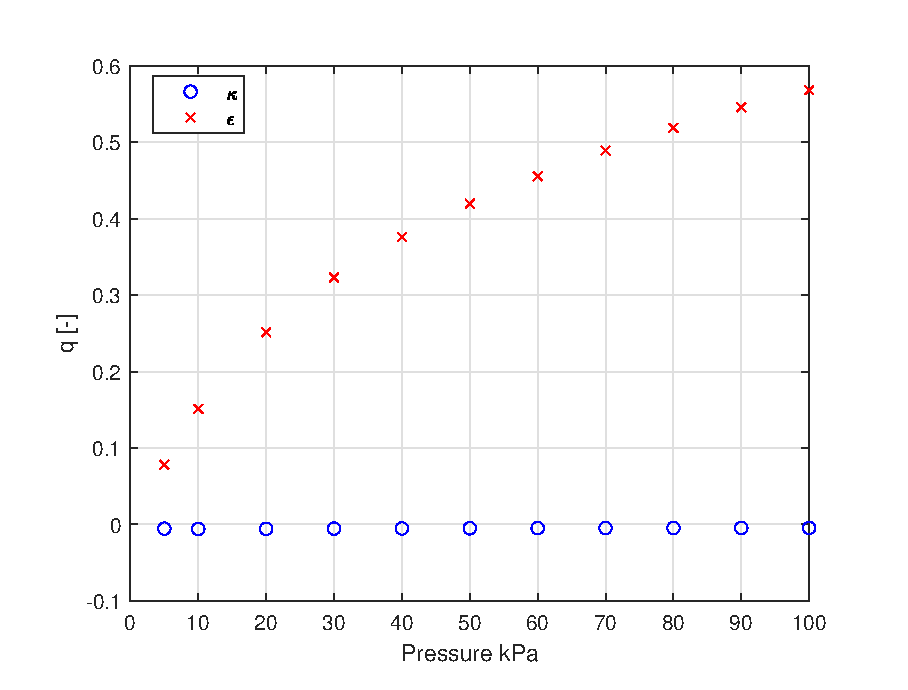
\includegraphics[width = 0.8\textwidth]{ProgressOverview/elongq.eps}
    \caption{Values for q as function of pressure}
    \label{fig:elongq}
\end{figure}


\begin{figure}[H]
    \centering
    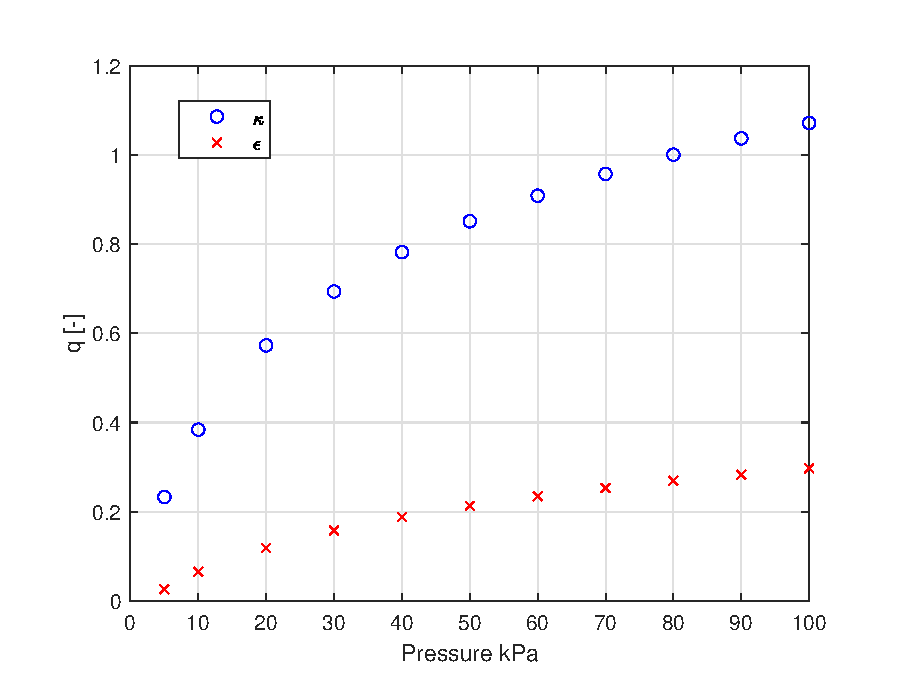
\includegraphics[width = 0.8\textwidth]{ProgressOverview/rotq.eps}
    \caption{Values for q as function of pressure}
    \label{fig:rotq}
\end{figure}